\section{Local disk model}
We study the local stability of an inviscid, self-gravitating and
magnetized fluid disk orbiting a central mass with
potential $\Phi_*(r,z)$, where $(r,\varphi,z)$ are cylindrical
co-ordinates from the central mass. We use the shearing box approximation     
\citep{goldreich65b} and consider a small patch of the disk at
$r=r_0$. The local frame rotates at angular velocity 
$\Omega_0=\Omega(r_0,0)$ about the central mass, where $r\Omega^2 =
\p\Phi_*/\p r$. We also define $S=-r\p\Omega/\p r$ as the local shear
rate and $\Omega_z^2\equiv\p^2\Phi_*/\p z^2$ as the square of the
local vertical frequency. 

A Cartesian co-ordinate system $(x,y,z)$ is set
up in this local frame, corresponding to the radial, azimuthal and vertical
directions of the global disk, respectively. The shearing box fluid
equations read 
\begin{align} 
  &\frac{\p\rho}{\p t}+\nabla\cdot(\rho\bm{v}) = 0,\\
  &\frac{\p \bm{v}}{\p t} + \bm{v}\cdot\nabla\bm{v} +
  2\Omega_0\hat{\bm{z}}\times\bm{v} = - \frac{1}{\rho}\nabla\Pi +
  \frac{1}{\rho\mu_0}\bm{B}\cdot\nabla\bm{B}
  -\nabla\Phi,\\
  &\frac{\p\bm{B}}{\p t}= \nabla\times\left(\bm{v}\times\bm{B} -
  \eta\nabla\times\bm{B}\right), 
\end{align}
where $\rho$ is the density field; $\bm{v}$ is the total velocity in
the local frame; $\bm{B}$ is the magnetic field which satisfies
$\nabla\cdot~\bm{B}=0$; $\Pi \equiv P +
|\bm{B}|^2/2\mu_0$ is the total pressure ($\mu_0$ is the vacuum
permeability). We choose a barotropic equation of state, specified
below, so that the gas pressure is given by $P=P(\rho)$. The
resistivity $\eta$ is either uniform or a prescribed function of
height. 
%The %resistivity is allowed to be non-uniform, $\eta=eta(z)$.  

%is the gas pressure given by a
%barotropic equation of state chosen later.  
%no curvature effects - magnetic tension neglected (limits strength of
%toroidal field that can be considered

The total potential is $\Phi = \Phi_\mathrm{ext} + \Phi_d$, where
\begin{align}
  \Phi_\mathrm{ext}(x,z) = -\Omega_0 S_0 x^2 +
  \frac{1}{2}\Omega_{z0}^2z^2 
\end{align}
is the effective external potential (central plus centrifugal) in the
shearing box approximation, where $S_0\equiv S(r_0,0)$ and
$\Omega_{z0}\equiv\Omega_z(r_0,0)$; 
%% \begin{align}
%%   S\equiv -r\frac{\p\Omega}{\p r}, \quad\quad \Omega_{z0}^2\equiv
%%   \frac{\p^2\Phi_*}{\p z^2} 
%% \end{align}
%is the local shear rate and vertical frequency respectively; 
and the gas potential $\Phi_d$ statisfies Poisson's equation
\begin{align}
  \nabla^2\Phi_d = 4\pi G \rho, 
\end{align}
where $G$ is the gravitational constant. For clarity, hereafter we
drop the subscript $0$ on the frequencies. 

%We consider two cases
%\begin{enumerate}
%\item Purely vertical field with constant or variable
%  resistivity, so that $\epsilon = 0$ and $\eta=\eta(z)$. 
%\item Tilted field with uniform resistivity
%  so that $\epsilon \neq 0$ and $\eta=\rm{constant}$.   
%\end{enumerate}

\subsection{Equilibrium disk} 
The unperturbed disk is steady and described by
$\rho=\rho(z)$, $\bm{B} = B_z\hat{\bm{z}} + B_y\hat{\bm{y}}$ where
$B_{y,z}$ are constants and the toroidal field strength is
$B_y=\epsilon B_z$. The equilibrium 
velocity field is $\bm{v} = -Sx\hat{\bm{y}}$. We consider Keplerian
disks so that $S = 3\Omega/2$ and the epicyclic frequency 
$\kappa\equiv\sqrt{2\Omega(2\Omega-S)}=\Omega=\Omega_z$. 
%$\Omega = \Omega_z.$ 
We assume a thin disk and neglect the radial component of the
self-gravitational force in 
the unperturbed disk.    

The equilibrium density field is obtained by solving
\begin{align}
  &0=\frac{1}{\rho}\frac{d P}{dz} + \Omega_z^2z + \frac{d\Phi_d}{dz},\label{eqm_eqns1}\\
  &\frac{d^2\Phi_d}{dz^2} = 4\pi G \rho.\label{eqm_eqns2}
\end{align}
We consider \begin{inparaenum}[(i)]
\item isothermal disks with $P=c_{s0}^2\rho$\label{iso_eos}; 
\item polytropic disks with $P=K\rho^2$ with $K=c_{s0}^2/2\rho_0$;
\end{inparaenum}
where $\rho_0\equiv\rho(0)$. The sound speed $c_s\equiv\sqrt{dP/d\rho}$
so that $c_{s0}$ is the global sound speed in the isothermal disk, and
is the mid-plane sound speed in the polytropic disk. For the polytropic
disk the disk thickness $H$ is such that $\rho(H)=0$. Since the
isothermal disk has no surface, we define $H$ such that
$\rho(H)=\epsilon\rho(0)$ with $\epsilon=10^{-2}$.   

%and $\rho_0\equiv\rho(0)$

We solve for $\hat{\rho}\equiv\rho/\rho_0$ with 
%$\rho_0\equiv\rho(0)$ is the mid-plane density.
%is parameterized via the
%Toomre $Q$ parameter such that $\rho_0=\Omega^2/4\pi G Q$. 
boundary conditions $\hat{\rho}=1$ and $d\hat{\rho}/dz=0$  at $z=0$. This
is done numerically for isothermal disks and analytically for the
polytropic disk (see Appendix \ref{appen1}). Examples of density
profiles are shown in Fig. \ref{eqm_den}. The normalized density field
is weakly dependent on the strength of self-gravity provided the
vertical co-ordinate is appropriately scaled as well.  

%As the strength of self-gravity increases, the
%disk becomes thinner ($H$ decreases)

%The isothermal disk shows that self-gravity
%compresses the disk and reduces the true pressure scale-height. The
%polytropic disk shows little difference between different strengths of
%self-gravity because the vertical co-ordiante is already normalized by
%the disk thickness. 

\begin{figure}
  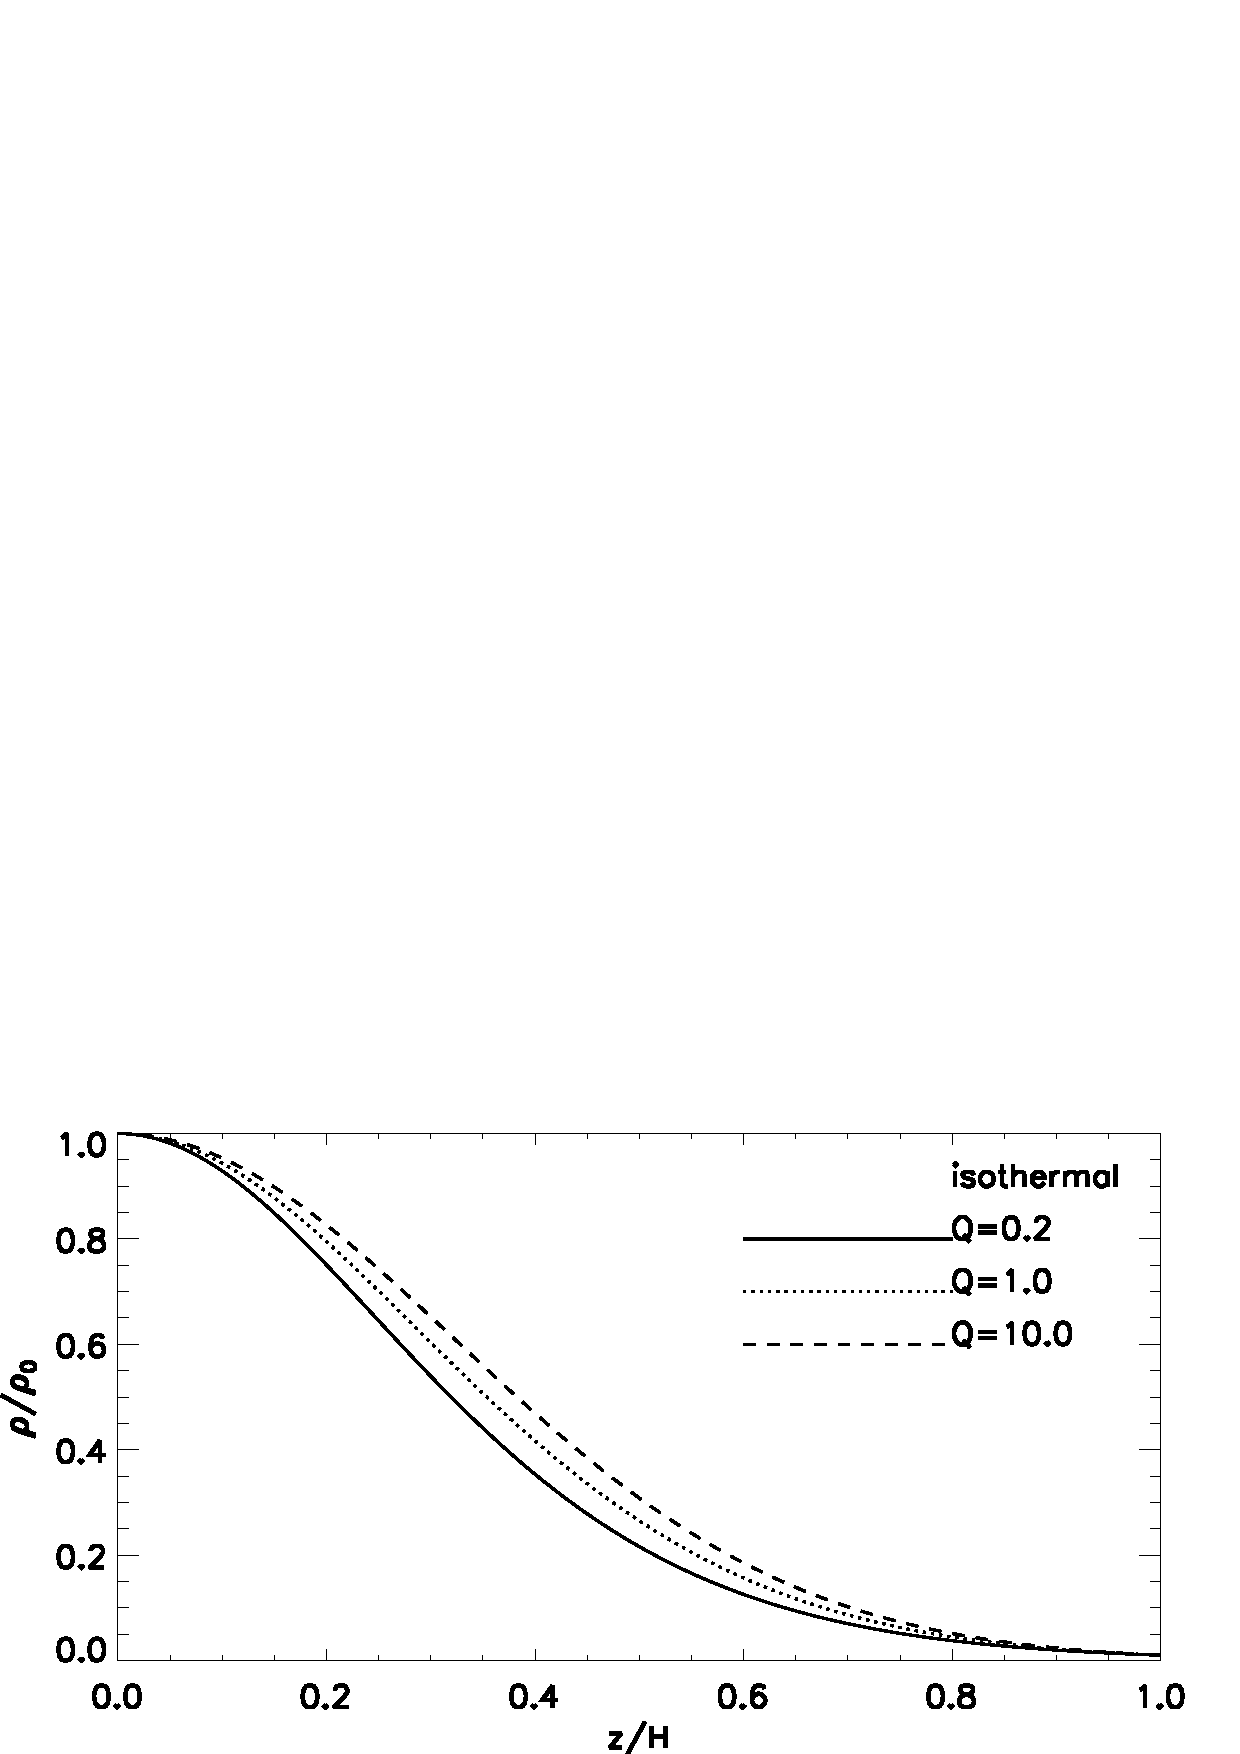
\includegraphics[width=\linewidth,clip=true,trim=0cm 1.5cm 0cm 0cm]{figures/compare_iso_density}
  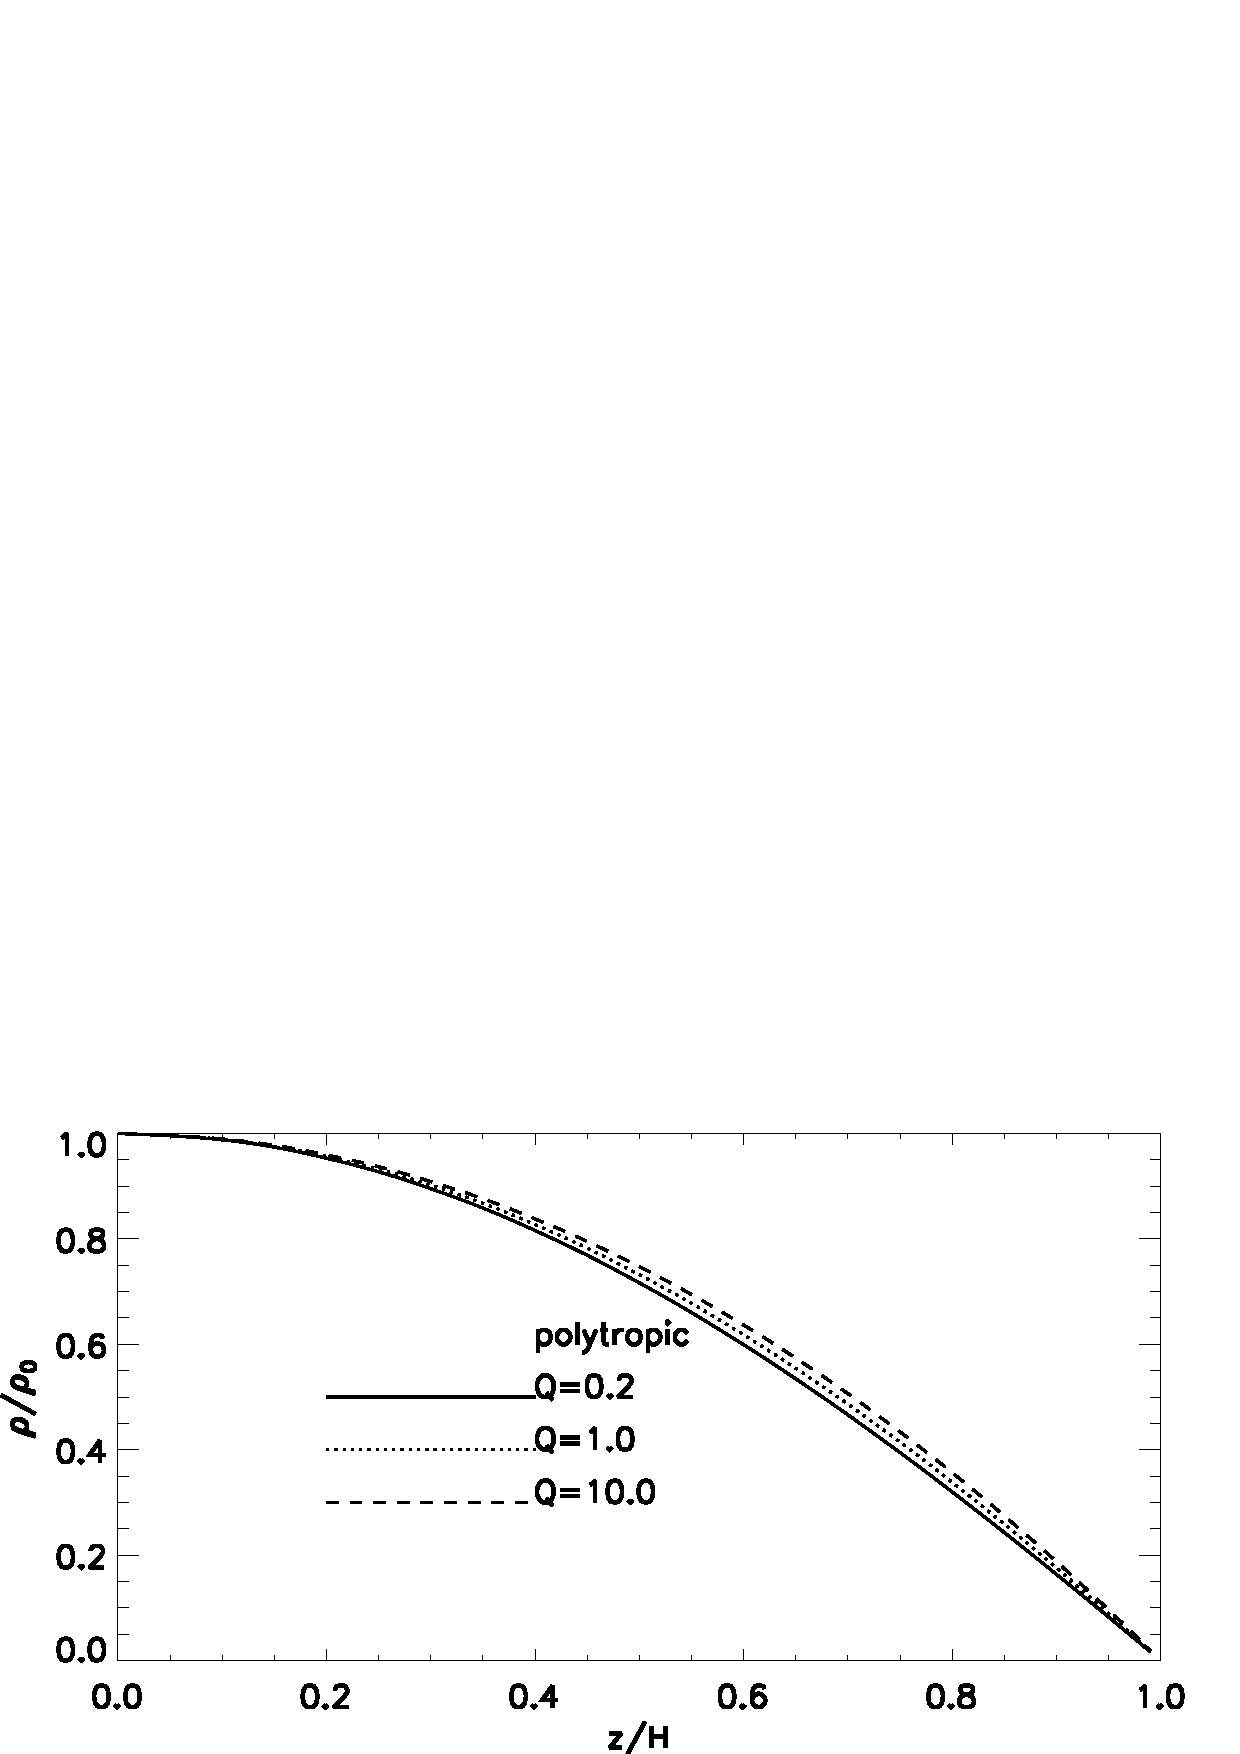
\includegraphics[width=\linewidth,clip=true,trim=0cm 0cm 0cm 0.9cm]{figures/compare_poly_density}
  \caption{Equilibrium density field from solving Eq. \ref{eqm_eqns1}
    --- \ref{eqm_eqns2} subject to an isothermal (top) and polytropic
    (bottom) equation of state. Note that the normalization for the
    horizontal axis also depends on the strength of self-gravity,
    i.e. $H=H(Q)$ and is a decreasing function of $Q$. 
%Note that the vertical co-ordinate is
%    normalized differently for convenience. In the isothermal disk,
%    $H$ is the characteristic scale-height in the
%    non-self-gravitating limit; in the polytropic disk $H$ is the
%    disk thickness. 
\label{eqm_den}}
\end{figure}

%\subsection{}




\subsection{Resistivity profile}\label{resis_profile}
In this work we consider either constant resistivity or a
resistivity prescription such that $\eta(z)$ increases away from the
midplane. In the latter case, we follow \cite{fleming03} and adopt the
resistivity profile 
\begin{align}
  \eta(z) =
  \sqrt{2}\eta_0\left[\exp{\left(-g_+\right)}+\exp{\left(-g_-\right)}\right]^{-1/2},  
\end{align}
where
\begin{align}
  &g_\pm(z) =  \frac{\Sigma_\pm(z)-\Sigma_0}{\Sigma_*}, \\
  &\Sigma_\pm(z) = \int_{\pm z}^\infty\rho(z^\prime)dz^\prime, \label{sigma_pm}
\end{align}
and $\Sigma_0\equiv\Sigma_{\pm}(0)$, so that $g_\pm(0)=0$ and $\eta_0 
= \eta(0)$. The constant $\Sigma_*$ is chosen such that 
\begin{align}
  \cosh{\left(\frac{\Sigma_0}{\Sigma_*}\right)} =
  \left[\frac{\eta_0}{\eta(\infty)}\right]^2,
\end{align}
and we define $\eta_0/\eta(\infty)\equiv A$ as the conductivity
boost factor from the midplane to the disk surface. We remark that
once the equilibrium $\rho$ and $d\rho/dz$ are obtained from
Eq. \ref{eqm_eqns1} --- \ref{eqm_eqns2}, the integration for
Eq. \ref{sigma_pm} can be performed implicitly by using Poisson's 
equation. 


We use the Elsasser number $\Lambda$ as a non-dimensional measure of
conductivity,
\begin{align} 
  \Lambda \equiv \frac{v_A^2}{\eta\Omega},
\end{align}
where $v_A \equiv B_z/\sqrt{\mu_0\rho}$ is the vertical Alfven speed. Example
profiles of $\Lambda$ are shown in Fig. \ref{eqm_resis} for the
isothermal disk. The disk may be considered ideal where $\Lambda
\gtrsim 1$. Since $\hat{\rho}(z/H)$ is weakly dependent on  self-gravity, the
ideal region only expands slightly as $Q$ is decreased. 

%A similar plot is obtained for polytropic disks.   

%The conductivity is boosted by a factor $A=10$ from the midplane to
%the upper disk boundary. The figure compares a strongly self-gravitating case
%($Q=0.2$) and the non-self-gravitating limit ($Q=10$). 

\begin{figure}
  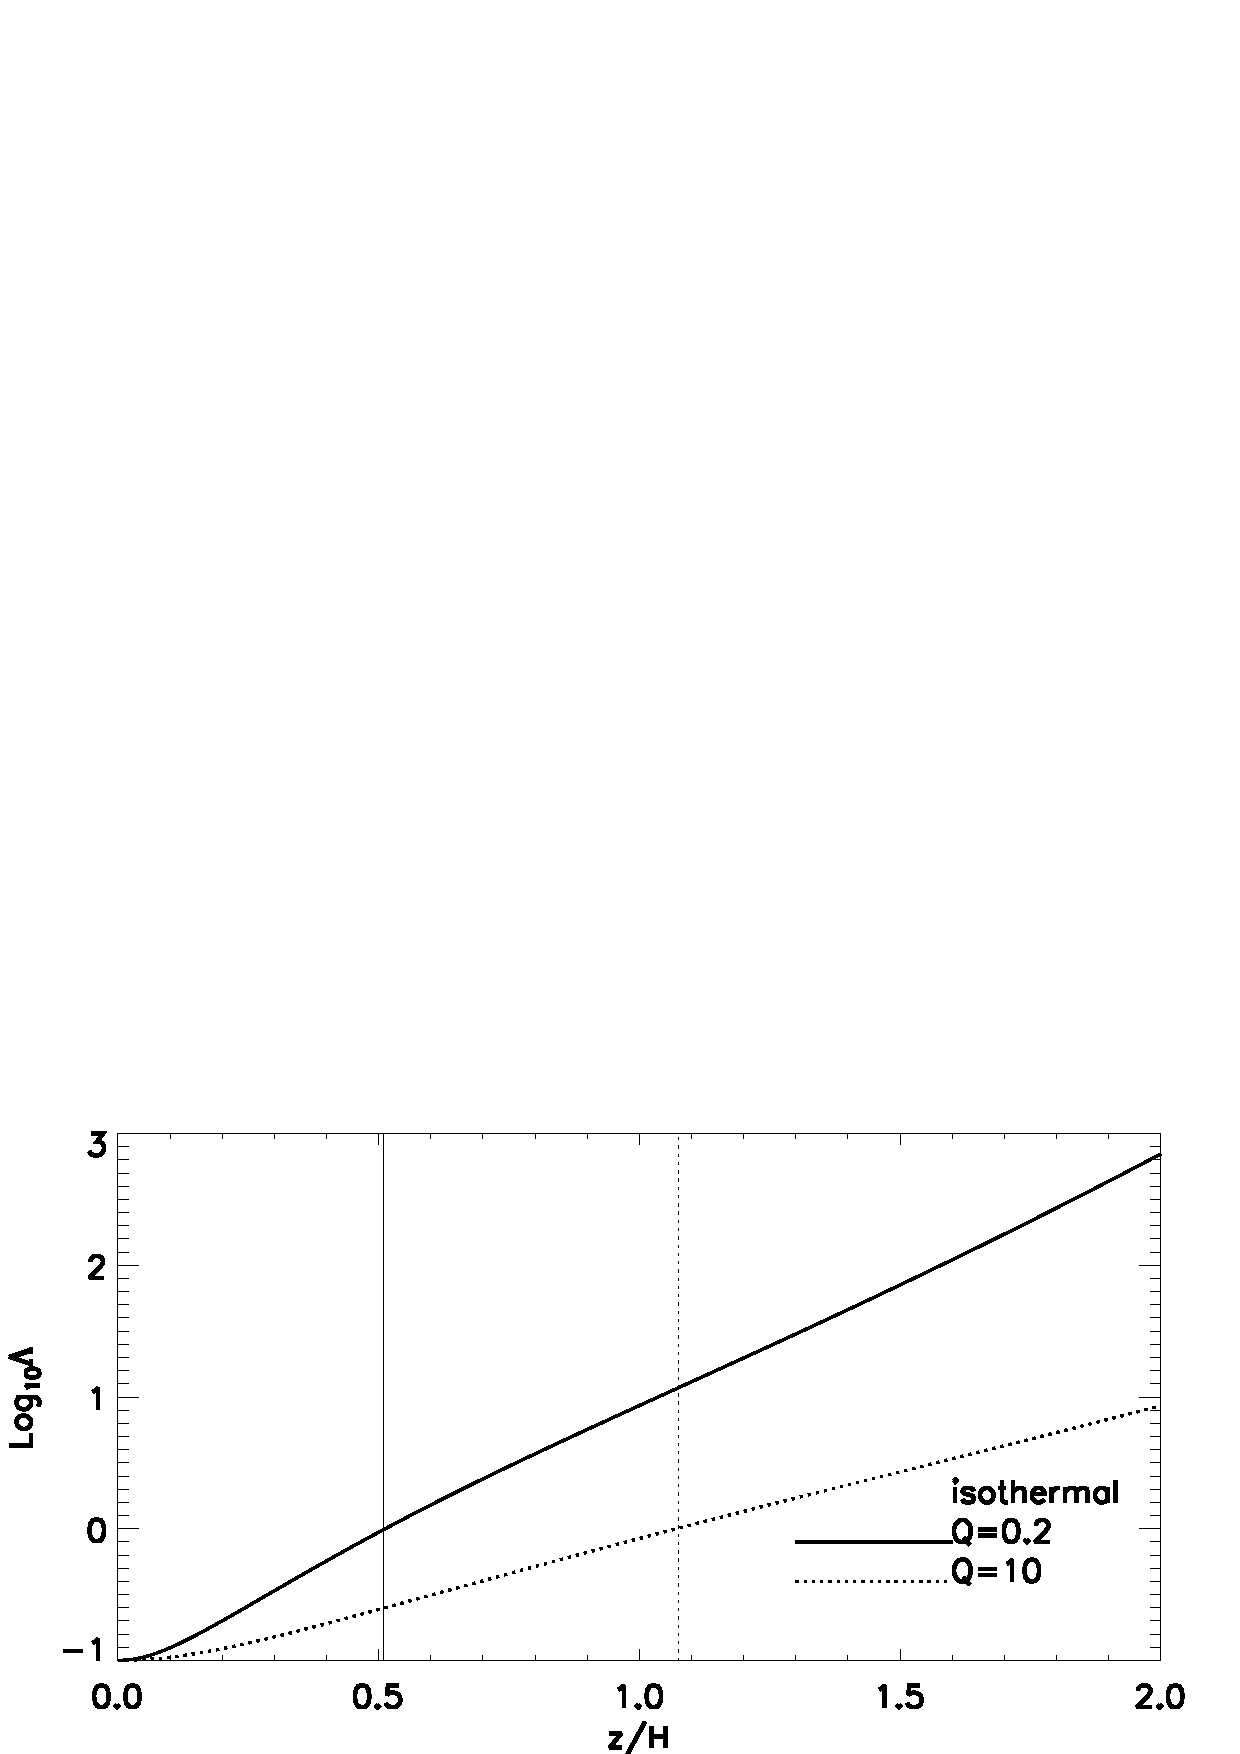
\includegraphics[width=\linewidth]{figures/elsasser_iso}
  \caption{Elsasser number as prescribed in \S\ref{resis_profile} for
    isothermal disks with $Q=0.2$ (solid) 
    and $Q=10$ (dotted). The vertical line
    indicates $\Lambda=1$ in each case. \label{eqm_resis}}
\end{figure}


\subsection{System parameters}
We summarize here the main parameters describing the resistive,
self-gravitating shearing box. The strength of self-gravity is
parametrized by 
\begin{align}
  Q \equiv \frac{\Omega^2}{4\pi G\rho_0}
\end{align}
\citep{mamat10}, which is used to set the mid-plane density $\rho_0$. 
The relation between $Q$ and the Toomre parameter for gravitational
instability of razor-thin disks is described in Appendix \ref{q3d2d}. 

The plasma $\beta$ measures the inverse strength of the  
magnetic field, 
\begin{align}
  \beta \equiv \frac{\csmid^2}{v_{A0}^2} =
  \frac{\csmid^2\mu_0\rho_0}{B_z^2},  
\end{align}
where $v_{A0}$ is the midplane Alfven speed. The strength of
resistivity is measured by the midplane Elsasser number 
\begin{align}
  \Lambda_0 \equiv\Lambda(0) =  \frac{v_{A0}^2}{\eta_0\Omega} = \frac{f^2 R_m}{\beta}, 
\end{align}
where the third equality defines the magnetic Reynolds number
$R_m=H^2\Omega/\eta_0$ and $f\equiv \csmid/H\Omega$ is a numerical
factor of order unity. 

%The Elsasser number as a function of height is $\Lambda(z)\equiv
%v_A^2/\eta\Omega$. 
